\section{RC Week 7}

\subsection{IO}
\begin{frame}[fragile]{Buffered Input streams}

The only input stream is \texttt{cin}, the standard input stream. The input stream is buffered.

\begin{enumerate}
	\item When you hit keyboard, the OS receives the keyboard key stroke and buffers what you type. \item You can always modify your input at this point.
	\item When you hit enter (or CTRL-C, etc.), OS sends the inputs to your program.
	\item Your program itself again buffers the input it receives.
	\item Read from your programs' buffer when you extract from \texttt{cin}.
\end{enumerate}	


It is somewhat useful to know that, when you hit enter, not only the your previous inputs are sent to the program, but also the "enter" keystroke it self. What is the ASCII character for the "enter" key?

If you are to write interactive programs, e.g. games that responds to direction keys, you will have to work with the underlying operating systems. 

\end{frame}

\begin{frame}[fragile]{How does input stream work?}
If we are to understand the behavior of input streams, we must turn to its internal workings. The input stream follows a 3 step procedure
\begin{enumerate}
\item Read the input stream character by character.
\item Based on the read characters, and target stop at some point.
\item Convert what you read into required type.
\end{enumerate}
We demonstrate on an example. Suppose you try to execute 

\begin{minted}{c++}
string stt; cin >> str;  // cin contains "123abc hello world"
\end{minted}

\begin{itemize}
\item Read the input stream until it hits a blank character.
\item The blank character remains in the stream. 
\item Trim the string, remove all leading blanks.
\item Copies the result into \texttt{str}.
\item The stream is left with \texttt{ hello world}, 1 leading space.
\end{itemize}
\end{frame}

\begin{frame}[fragile]{How does input stream work? Cont'}
The following is a summary of usually behaviors of common behavior extraction operators. \textbf{based on my memory}. Suppose:
\begin{minted}{c++}
T var; cin >> var;
\end{minted}
\begin{itemize}
\item If \texttt{T} is numeric types, such as \texttt{int}. 1) First character might be the sign. 2) Reads until the first non-digit character 3) The non-digit character is left in the stream. 
\item If \texttt{T} is \texttt{char}. It extracts exactly one character from the stream, no matter what that character is. Equivalent to \texttt{getch()}.
\item if \texttt{T} is \texttt{char*}. It do exactly as the string. In the final step it copies the characters read to where the pointer points. \textit{It is dangerous because of buffer overflow.}
\end{itemize}

\begin{minted}{c++}
istream& getline(istream& is, std::string& str);
\end{minted}

This function 1) Reads from the stream \texttt{is} 2) Stops until a newline character. 3) The encountered new line character is \textbf{extracted out, but ditched} (not copied into \texttt{str}) 
\end{frame}

\begin{frame}[fragile]
\frametitle{Avoid parsing whenever possible!}
Specifically, avoid using \texttt{getline()} and \texttt{getch()} whenever possible. The C++ extractors has a very nice property: if you try to extract numbers or strings, the extractor automatically ignores blank characters. This means you only need to focus on the question of 
\begin{center}
\textit{WHAT is the next thing I need?}
\end{center}

instead of thinking 
\begin{itemize}
\item WHERE is the next thing I need?
\item Is what I need on the next line?
\item Is there a space or a tab before what I need?
\item How do I get rid of that space / tab / newline?
\end{itemize}
\end{frame}

\begin{frame}[fragile]
\frametitle{The failed state}
If you try to extract invalid things from the stream, the stream enters a so called \textit{Failed State}. 

Two typical situation where a input stream will enter a fail state is when you try to extract things from an empty stream (all things in the stream has be extracted). Or you extracted the wrong type.

In general the second situation should be avoided. If you are not sure what next thing is, use a string to accept it. Transform the string into expected type later.

You can test whether a stream is in a valid state (very often if there is still thing remains in the stream) by simply \texttt{if(stream)}.

A very commonly used idiom to extract everything is:

\begin{minted}{c++}
int num; while(cin >> num) /* Do something here */;
\end{minted}

Please note that extractor operator returns an reference of the left hand stream.
\end{frame}

\begin{frame}[fragile]{Buffered Output Streams}
There are 2 output streams \texttt{cout} and \texttt{cerr}

\begin{itemize}
\item \texttt{cout} is the standard output stream. It is buffered. 
\item \texttt{cerrr} is the standard error stream. It is NOT buffered. 
\end{itemize}

File outputs are almost always buffered. If an output stream is buffered, it usually works as follows.

\begin{itemize}
\item Your program stores the output in a buffer.
\item When the buffer is full, or explicitly flushed, your program sends the buffer content to OS.
\item The OS puts the content into a file, or onto the screen (which is also a ``file", remember?).
\item Inserting a \texttt{std::flush}, or \texttt{std::endl} flushes the buffer.
\end{itemize}

Standard output streams accepts normal program outputs. On the other hand, \texttt{cerr} accepts error messages, \textbf{warnings} and \textbf{diagnostic messages}. 
\end{frame}

\begin{frame}[fragile]{Buffer, flush and performance}

\textit{Buffering} have a few implications, or more likely problems. 

\begin{itemize}
\item If your program crashed at some point, information in the buffer will be lost and thus not print out (for this reason \texttt{cerr} is not buffered).
\item There is an extra overhead of maintaining the consistence of the C++ style streamed IO with C style \texttt{printf}, \texttt{puts}... 
\end{itemize}

And there's more to it. Although \texttt{cout} and \texttt{cerr} are two different streams, they usually both goes to the stream.  If you output to both of them, for example

\begin{minted}{c++}
cout << "Hello "; cerr << " Gotcha "; cout << "World!"
\end{minted}

It is possible you see any one the following three (why?): 1) \texttt{Hello Gotcha World!} 2) \texttt{Gotcha Hello World?} 3) \texttt{Hello World! Gotcha}. What to do if I want to ensure the order?
\end{frame}


\begin{frame}[fragile]{Buffer, flush and performance, Cont'}

Why do we need such buffer? If it causes so many problems? 

The reason is actually performance, flushing the buffer, or printing things onto the screen requires an interaction with the operating system, which is very expensive!

Buffer is an attempt reduce the number of such interaction by trying to send as much text as possible out at once. Compare:

\begin{minted}{c++}
for (int i=0; i<10000; i++) cout << "Hello" << endl;
for (int i=0; i<10000; i++) cout << "Hello" << "\n";
\end{minted}

Generally the first one could be at least 3 times slower than the second one. This will be significant in the runtime of your program since your projects are often IO heavy (outputs a lot).
\end{frame}

\begin{frame}[fragile]{Type signature of extraction / insertion operators}
The reason why C++ iostream can work seamlessly with various types, is because it uses operator overloading and inheritance. The type signature of the extraction operator (often) has the following type (general) signature.

\begin{minted}{c++}
istream& operator>>(istream& is, T& var); 
ostream& operator<<(ostream& os, const T& var);  
\end{minted}

The standard library provides the following for \texttt{std::string}s. 
\begin{minted}{c++}
istream& operator>>(istream&, std::string&); 
ostream& operator<<(ostream&, const std::string&);
\end{minted}

For smaller types, insertion operator may accept pass-by-values, not const references.
\begin{minted}{c++}
istream& operator>>(istream& is, int& var); 
ostream& operator<<(ostream& os, int var);
\end{minted}


\end{frame}

\begin{frame}[fragile]{Type signature of extraction / insertion operators, cont'}

\begin{minted}{c++}
istream& operator>>(istream& is, T& var); 
ostream& operator<<(ostream& os, const T& var);
\end{minted}

\begin{itemize}
\item Each type that supports extraction has its own overloading of the function. 
\item All sources that supports character-by-character reading inherits from \texttt{istream}. For example, the input file stream \texttt{ifstream}.
\item For extraction operator, variable is passed by reference, allows putting the value ``into" the variable. 
\item For insertion operator, variable is passed often by \textbf{const reference}. Why?
\item The operator returns first argument as its return value. This allows ``chaining" the extraction / insertion. 
\item Functions like \texttt{getline()} also follows this convention. 
\end{itemize}
\end{frame}

\begin{frame}[fragile]{Chaining extraction / insertion operator}
A C++ beginner always quickly get used to write things like:
\begin{minted}{c++}
int x, y; char c1, c2; std::string str; 
getline(cin >> x >> c1, str) >> c2 >> y;
\end{minted}
The syntax is very concise compared to C (\texttt{fscanf()}). The question is, how does it work, without specifying the format string?

The secret is mainly lies in the type signature of extraction operators, specifically:
\begin{itemize}
	\item Extraction (insertion) operators are left associative, meaning parentheses are grouped left to right.
	\item Compiler chooses overloads according to the second argument. This avoids the \texttt{scanf()} style format string. 
	\item Operators return a reference to the stream. 
\end{itemize}
Remark: this example demonstrates what is known as \textit{static polymorphism}, where the identical code is resolved to different function calls at compile time.
\end{frame}

\begin{frame}[fragile]{Chaining extraction / insertion operator, Cont'}
We apply parentheses to previous example:
\begin{minted}{c++}
(getline(((cin >> x) >> c1), str) >> c2 )>> y;
\end{minted}
The first thing to evaluate the is the argument of \texttt{getline(...)}. Note that \texttt{cin} is of type \texttt{istream}, \texttt{x} is of type {int}. The compiler chooses overload:
\begin{minted}{c++}
istream& operator>>(istream& is, int& var);  
\end{minted}
It takes \texttt{cin} as \texttt{is}, \texttt{x} as \texttt{var}. After extracting one integer from \texttt{cin} it again returns the reference of \texttt{cin}. 
\begin{minted}{c++}
((...) /* Evaluates to cin */ >> c1)
\end{minted}
This allows the compiler to deduce the second overload for \texttt{c1}. 
\begin{minted}{c++}
istream& operator>>(istream& is, char& var);  
\end{minted}
This goes recursively on and on. It should now also be clear why \texttt{getline()} should return a reference to its first argument. 
\end{frame}

\begin{frame}{Writing a tree to standard output}
This is a code snippet from the VE280 Online judge code that write a tree to standard output.  A tree is can be written out in the form \texttt{[ tree\_elt [\{left\_tree\}] [\{right\_tree\}] ]}. For example \texttt{[ 2 [ 1 \$ [ 3 \$ \$ ] ] [ 1 [ 4 \$ \$ ] [ 6 \$ \$ ] ] ]}. The \texttt{\$} represents empty tree.

File: \texttt{code/rc7writetree/writetree.cpp}
\inputminted[]{c++}{code/rc7writetree/writetree.cpp}
\end{frame}


%\begin{frame}[fragile]{Tips on working with input stream}
%\framesubtitle{A VG101 Problem}
%Recall the following VG101 problem (guess lots of you suffered...):
%\begin{figure}
%\centering
%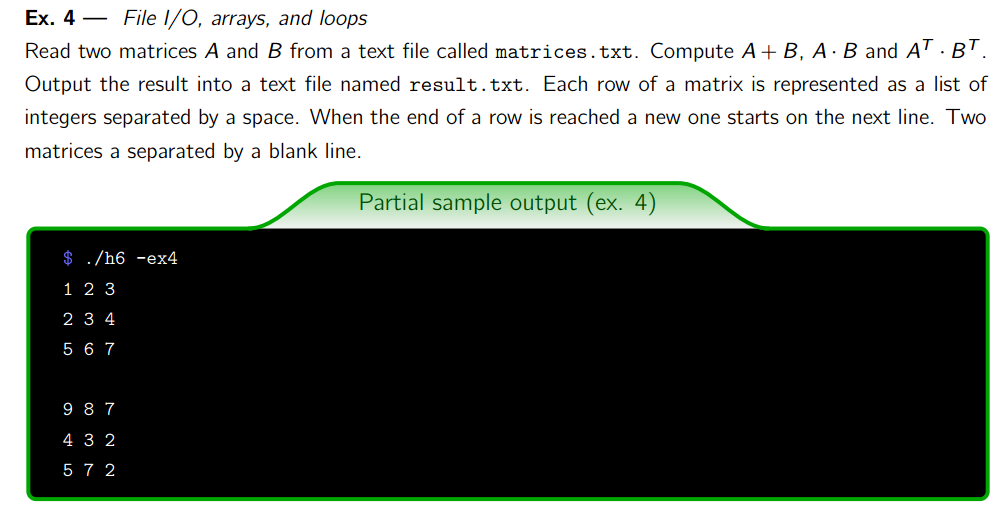
\includegraphics[scale=0.4]{fig/rc5_vg101}
%\end{figure}
%\end{frame}

\begin{frame}[fragile]{Tips on working with file streams}
File streams are very much like \texttt{cin} or \texttt{cout}. Please note the difference of \texttt{ifstream} and \texttt{ofstream} and \texttt{fstream}. 

File streams can be opened on construction:
\begin{minted}{c++}
ifstream inputFileStream("input.txt");
\end{minted}
Above code opens \texttt{input.txt} with a \texttt{ifstream}. Please note if the file doesn't exist or failed to open, your \texttt{inputFileStream} will be in a failed state. Remember to check!

Although you can use \texttt{inputFileSteam.close()} to close the stream (and clear its buffer), but you don't actually need to. Remember the stack unwinding example we have before? Standard libraries' file stream are exactly such objects. Its deconstructor will take care of the closing and freeing the file.
\end{frame}

\begin{frame}[fragile]{Use \texttt{istringstream} as parser }
A \texttt{stringstream} can either act be an input stream, or an output stream. They are very different! 

\texttt{istringstream} needs to be ``attached" to a string. This can be down by either passing the string in on construction or use its \texttt{.str()} method. The stringstream, unlike \texttt{cin}, doesn't consume the string, instead it attach a ``pointer" to the string. Ideally:

\begin{minted}{text}
123 abc def Hello world  |  123 abc def Hello world
|<-sstream               |     |<-sstream 
\end{minted}

Right side is after extracting 123 through \texttt{sstream >> intVar;}

\texttt{istringstream} is especially useful in treating data acquired from \texttt{getline}. 

\alert{If you need to use the same \texttt{istringstream} object for multiple strings, you need to clear it when changing string}. 
\end{frame}

\begin{frame}[fragile]{Use \texttt{ostringstream} as string builder}
From time to time we need to convert different type of data into a string. For example, information about a student is described by:
\begin{minted}{c++}
strcut Student {
string name; int grade; Date birthday; double GPA;
};
\end{minted}
And you need to turn such stuctures into below format
\begin{minted}{c++}
%name, %grade grade, %YYYY-MM-DD, gpa = %gpa"
\end{minted}
You can setup an \texttt{ostringstream}. You simply push into the stream as if it is \texttt{cout}, finally you call \texttt{ostringstream.str()} to get the result. 
\begin{minted}{c++}
oss << name << "," << grade << " grade" << ... 
\end{minted}
The design of the stream makes it very efficient in dealing with large amount of text. For example you can use it to prepare data to send over the Internet.
\end{frame}

\subsection{Data Abstraction with \texttt{class}es}
\begin{frame}{Once another look on data types: Duck typing}
Consider the problem: 
\begin{center}
	\structure{Define what a ``Duck" is?}
\end{center}
The very answer from \textit{Alex Martelli} is:
\begin{quotation}
	In other words, don't check whether it IS-a duck: check whether it QUACKS-like-a duck, WALKS-like-a duck, etc, etc, depending on exactly what subset of duck-like behaviour you need to play your language-games with.
\end{quotation}
The whole purpose of having data type is to model things. We use \texttt{struct} to model what something consists. But things are only useful when we interact with them. The \textit{observable} effects are all we care. \alert{The whole point of data abstraction is to model the behavior of objects}.
\end{frame}

\begin{frame}{Abstract Data type}
The central idea is:
\begin{center}
\structure{Data type IS Abstraction.}
\end{center}
Always define a datatype in terms of what it can do, what kind of operations are supported for this datatype, and \alert{there should be nothing more}. Also define what you \alert{CANNOT} do with such data.
\begin{description}[Information Hiding]
\item[Information Hiding] Actual implementation of the object is hidden away, the outside can't see, and shouldn't see what's inside.
\item[Encapsulation] Operations become part of the type. 
\item[Locality] Other components only depend on exposed operations (i.e. interfaces), nothing more. This is different for \texttt{struct}.
\item[Substitutable] Change the implementable preserves program correctness.
\end{description}
\end{frame}

\begin{frame}[fragile]{Designing ADTs with \texttt{class}es}
We would like specify an Integer class:
\begin{columns}[]
\column{.5\textwidth}

\vspace{-.2in}
\begin{minted}{c++}
class Natural {
// OVERVIEW: An N
public:
void  set(int v);
// EFFECT:  ...
// MODIFIES: this
Natural  add(Natural v);
Natural  mul(Natural v);
int get();
private:
int value;
};
Natrual num;
\end{minted}
\column{.6\textwidth}

\vspace{-.2in}
\begin{itemize}
\small
\item \texttt{class} key word begins the specification of an abstract datatype. CamelCase style recommand you to capitalize first character.
\item \texttt{public} key words begins specifying the \textit{operations}, the \textit{abstaction}, or we say the \textit{interface}. Pay attention to the \texttt{MODIFIES: this}.
\item \texttt{private} key words calls for actual implementation.
\item Note what's not there: a \texttt{div} method. Dividing natural numbers usually don't give you natural numbers.
\item \texttt{num} is called an \textit{object}. \texttt{num} is an \textit{instance} of \texttt{Natural}. 
\end{itemize}
\end{columns}
\end{frame}

\begin{frame}{Implementing \texttt{class}es}
We now need to try to implement a class. We focus especially implementing class methods (member functions are usually called \textit{methods}.). 

\vspace{0.1in}
The declaration of a class is usually written in a \textit{header file}. For the example of last page we usually implement it in \texttt{natural.h}. The name of the file usually is the same as the class you are implement.  

\vspace{0.1in}
Class methods can be implemented either when you declare the class, or in a separate \texttt{.cpp} file. For our above example we usually implement it in the \texttt{natural.cpp}.

\vspace{0.1in}
Whenever you need to use a class, you include its header file. Usually each header file only contains definition of one single class, unless you have a couple of tightly related class. 
\end{frame}

\begin{frame}[fragile]{Implementing \texttt{class}es}
\begin{columns}[]
\column{.5\textwidth}

\vspace{-.3in}
\begin{minted}{c++}
// Natural.h
#ifndef __NATURAL_H__
#defein __NATURAL_H__
class Natural {
public:
void  set(int v) {
this->value = v;
}
Natural  add(Natural v);
Natural  mul(Natural v);
int get() {return value;}
private:
int value;
};
#endif __NATURAL_H__
\end{minted}

\column{.5\textwidth}

\vspace{-.3in}

\begin{minted}{c++}
// Natural.cpp
#include "natural.h"
Natural 
Natural::add(Natural v) {
Natural n; 
n.set(value + v.get());
return n;
}

Natural 
Natural::mul(Natural v) {
Natural n; 
n.set(value * v.get());
return n;
}
\end{minted}
\end{columns}
\end{frame}



\begin{frame}[fragile]{A remark on \texttt{private}}
\texttt{private} means private to class, not to instance. 
\begin{columns}[]
\column{.42\textwidth}

\vspace{-.2in}
\begin{minted}{c++}
class Human {
int leg;
public:
int swapLeg(Human& h) {
swap(this->leg, h.leg);
}
int setLeg(int n) {
this->leg = n;
}
};
Human h1; h1.setLeg(10);
Human h2; h2.setLeg(3);
h1.swapLeg(h2);
\end{minted}

\column{.65\textwidth}

\vspace{-.2in}
\begin{itemize}
\item Code on the left compiles and runs without problem.
\item It's sometimes called "Since we are both human why can't I swap my leg to yours" effect.
\item This indicates the design choice that \texttt{private} is a technique to hide abstraction implementation, other than to prevent outside modification. 
\item Members are \alert{\texttt{private} by defualt} in a \texttt{class}. Recall that \texttt{struct} are just \texttt{class} whose member are by default \texttt{public}
\end{itemize}
\end{columns}
\end{frame}

\begin{frame}[fragile]{\texttt{this} keyword}
\begin{columns}[]
\column{.5\textwidth}

\vspace{-.3in}
\begin{minted}{c++}
class Natural {
int value;
public:
int get() { 
return value;
}
void set(int value) {
this->value = value;
}
void printThis() {
cout << this << endl;
}
// Omit other method
};
\end{minted}

\column{.5\textwidth}

\vspace{-.3in}
\begin{minted}{c++}
int main() {
Natrual n1; 
n1.printThis(); 
cout << &n1 << endl;
Natrual n2; 
n2.printThis();
cout << &n2 << endl;
}
\end{minted}

One \alert{possible} output:

\begin{minted}{text}
0x7ffff1fd2820
0x7ffff1fd2820
0x7ffff1fd2830
0x7ffff1fd2830
\end{minted}

Source under \texttt{code/rc8this}

\end{columns}
\end{frame}

\begin{frame}[fragile]{\texttt{this} keyword}
\begin{columns}[]
\column{.45\textwidth}

\vspace{-.3in}
\begin{minted}{c++}
class Natural {
int value;
public:
int get() { 
return value;
}
void set(int value) {
this->value = value;
}
void printThis() {
cout << this << endl;
}
// Omit other methods
};
\end{minted}

\column{.6\textwidth}
\vspace{-.2in}
\begin{itemize}
\item Non-static methods always have a \texttt{this} pointer available.
\item For non-const member methods \texttt{this} keyword is of type \texttt{ClassType*}.
\item Members (including methods) are \alert{always} accesses through \texttt{this} keyword, either explicitly (in \texttt{set()} method), or implicitly (\texttt{get()} method).
\item If there is an ambiguity you can use \texttt{this} to resolve ambiguity. In the \texttt{set} method, LHS refers to member and RHS refers to the argument.
\end{itemize}
\end{columns}
\end{frame}

\begin{frame}[fragile]{\texttt{const} member function and ripple effect}
A member function can be declared as \texttt{const} to signify it will not change any member (in any possible way). The declaration must be done both in the declaration and in the implementation:

\begin{columns}
\column{.45\textwidth}

\vspace{-.25in}
\begin{minted}{c++}
// useless_class.h
class UselessClass {
int value;
public:
int get() const;
};
\end{minted}

\column{.55\textwidth}

\vspace{-.25in}
\begin{minted}{c++}
// useless_class.cpp
int UselessClass::get() const {
return value;
}
\end{minted}
\end{columns}

\begin{itemize}
\item \texttt{const} methods cannot modify any member
\item \texttt{const} methods may only invoke other \texttt{const} methods.
\end{itemize}
You already know the basic rules of \texttt{const} methods. But unfortunately the situation (you will be facing) is much complicated (when you get to STLs). We now make a further discussion. 
\end{frame}

\begin{frame}[fragile]{\texttt{const} member function and propagation}
To illustrate the problem, we here uses a functionality called \textit{Runtime Type Info (RTTI)} to let the compiler spit out the types.

\texttt{* code/rc8const/main.cpp}
\inputminted[fontsize=\small, baselinestretch=0.865]{c++}{code/rc8const/main.cpp}	
\end{frame}

\begin{frame}{\texttt{const} member function and ripple effect}
We take down (and translate for you) the output of the program
\begin{description}[\texttt{bar()::value}]
\item[\texttt{bar()::this}] \texttt{const} pointer to \texttt{Foo}
\item[\texttt{bar()::value}] \texttt{const} pointer to \texttt{int}
\item[\texttt{baz()::this}] pointer to \texttt{Foo}
\item[\texttt{baz()::value}] pointer to \texttt{int}
\end{description}
Essentially we have the following 3 rules:
\begin{itemize}
\item In a \texttt{const} method, \texttt{this} have type \texttt{const Class*}
\item Non \texttt{const} member functions are not allowed to be accessed from a \texttt{const} object.
\item Any member variable accessed through a \texttt{const}ed \texttt{this} keyword is automatically const quantified.
\end{itemize}
We provide some examples to explain them.
\end{frame}

\begin{frame}{\texttt{const} member function and ripple effect}
We take down (and translate for you) the output of the program
\begin{description}[\texttt{bar()::value}]
\item[\texttt{bar()::this}]  pointer to \texttt{const Foo}
\item[\texttt{bar()::value}] pointer to \texttt{const int}
\item[\texttt{baz()::this}] pointer to \texttt{Foo}
\item[\texttt{baz()::value}] pointer to \texttt{int}
\end{description}
Essentially we have the following 3 rules:
\begin{itemize}
\item In a \texttt{const} method, \texttt{this} have type \texttt{const Class*}
\item Non \texttt{const} member functions are not allowed to be accessed from a \texttt{const} object.
\item Any member variable accessed through a \texttt{const}ed \texttt{this} keyword is automatically const quantified.
\end{itemize}
They seems very abstract. We provide some examples to explain them.
\end{frame}

\begin{frame}[fragile]{\texttt{const} ripple effect: Example }
Consider the following 2 classes
\begin{columns}

\column[]{.4\textwidth}
\vspace{-.2in}
\begin{minted}{c++}
class Integer {
int value;
public:
int get();
void set(int i);
};
\end{minted}

\column[]{.6\textwidth}
\vspace{-.2in}
\begin{minted}[]{c++}
class Bar {
Integer i;  Complicated c;
void doComp(); // uses c
public:
int getValue() { 
doComp(); return i.get(); 
} };
\end{minted}
\end{columns}

Suppose there exists a function that originally looks like:
\begin{minted}{c++}
void baz(Bar bar); // Do complicated work
\end{minted}
The function passes \texttt{Bar} by value. It was alright, until bar becomes really large. A quick fix is proposed. Somehow you know function does not modify the argument, you suggest to change it to 
\begin{minted}{c++}
void baz(const Bar& bar); // Do complicated work
\end{minted}
Pretty harmless change? What could be possibly go wrong?
\end{frame}

\begin{frame}{\texttt{const} ripple effect: Example}
Well it isn't! Let's see what happens:
\begin{itemize}
\small
\item We know \texttt{baz} calls \texttt{getValue} from \texttt{Bar} class. Since we change the argument to const reference. We can no long do that, since you cannot call a non-const member function on a const object.
\item You change \texttt{Bar::getValue()} to const member function. But this gives you 2 more problems (what are they?).
\item You tackle the easier one. Since \texttt{i} in \texttt{Bar::getValue()} is now const object, you have to change \texttt{Integer::get()} also to const member function.
\item Another problem is \texttt{doComp()} is not const. This function does really complicated calculation with \texttt{i} and \texttt{c}. 
\item You have no choice but to mark \texttt{Bar::doComp()} as const. This forces you inspect every member function of \texttt{Complicated} class, and change them to \texttt{const}.
\item Now you realize this will never end! There are simply more and more things to change. You ends up rewriting the entire code base! 
\end{itemize}
\end{frame}

\begin{frame}[fragile]{\texttt{const} ripple effect: Example}
Things you observed is sometimes called the ``ripple effect" of \texttt{const} keyword: when you change $X$, you ends up changing all things related to $X$, and this goes on and \texttt{const} ends up ``infecting" everything.

There are in general 2 ways to stop this effect, both of them are dangerous and far from satisfaction.
\begin{itemize}
\item A \texttt{const\_cast}. The programmer explicitly asks the compiler to stop checking constness and tell the compiler to trust him. 
\item Make a non-const copy of the original object. Pass that object along. This has a obvious performance drawback.
\end{itemize}

The lesson behind this is you \alert{constness is a all-or-nothing deal}. You either do it from the begging till the end, and never at all. Constness is considered good practice. It provides very powerful assurance on correctness. So our advice is simple:
\begin{center}
\alert{Do \texttt{const}, and do it in full scale!}
\end{center}
\end{frame}

\begin{frame}{Building source file containing classes}
We now turn to ask the question how classes are compiled. This is important for the following two reasons:
\begin{itemize}
\item How classes are compiled are related to the memory representation of classes. Many design choices on classes are (or were) have something to do with this.
\item You could encounter various strange problem in your project or in a real life situation. Knowing them helps to grasp the situation. 
\end{itemize}
Historically C++ was derived from a language called \textit{C With Classes}. One of the first C++ compiler will first translate C++ code into C code, then a C compiler compiles it into machine code. 

\vspace{0.03in}
We will notice that classes are (once were) merely C structures with some syntax sugar. We will also begin to notice how much trouble does the C linking strategy introduce into the language, and becomes prominent problem in its course of development. 
\end{frame}

\begin{frame}[fragile]{On compiling classes}
The code on the left will be compiled, as if, it was written in the form of the right hand side

\begin{columns}

\column{.5\textwidth}
\vspace{-.2in}
\begin{minted}[baselinestretch=.9, fontsize=\small]{c++}
class Clock {
int hour;
public:
void setHour(int h) {
hour = h;
}
int getHour() const {
return hour;
}
};
void foo() {
Clock clock; 
clock.setHour(10);
clock.getHour(); 
}
\end{minted}

\column{.5\textwidth}
\vspace{-.2in}
\begin{minted}[baselinestretch=.9, fontsize=\small]{c}
typedef struct Clock_t {
int hour; 
} Clock;
void clock_setHour
(Clock* this, int h) {
this->hour = h;
}
int clock_getHour
(const Clock* this) {
return this->hour;
}
void foo() {
Clock clock; 
clock_setHour(&clock, 10);
clock_getHour(&clock); 
}
\end{minted}
\end{columns}
\end{frame}

\begin{frame}{On compiling classes}
Now you should find the pattern:
\begin{itemize}
\item Classes are arranged in memory exactly like structures. We used to say ``structures are just classes whose members are all public". On a memory point of view, it's the other way around.
\item \alert{Methods are compiled into usual functions}, with one extra argument, the \texttt{this} keyword.
\item Dot operator (e.g. \texttt{clock.setHour}) are translated into usual function calls.
\item All members are accessed through the this parameter. The reason is now obvious.
\item \texttt{const} methods results in a \texttt{const} \texttt{this}.
\item \texttt{static} methods (if you still remember what they are), are just methods that does not take the extra argument (thus they are shared among all instances).
\end{itemize}
\end{frame}

\begin{frame}{On compiling classes: Linking}

We first go over a few things we already know about the building process (and see which of them are violated!):
\begin{itemize}
\item Building process is mainly about compiling and linking
\item Each source file compiles independently.
\item Each entity must have one definition and one only (ODR).
\end{itemize}

We have looked at  look at the linking stage. 

\vspace{.05in}
Remember information about classes are ``thrown away" in the compiling stage. When it comes to linking, we are only linking function calls together. Functions are all that we care.

\vspace{.05in}	
Every class method will be turned into a function. We keep that in mind and see the following slides.
\end{frame}

\begin{frame}[fragile]{On linking classes: the setup}
\begin{columns}
\column{.45\textwidth}

\vspace{-.25in}
\texttt{[code/rc8class/integer.h]}
\inputminted[fontsize=\small, baselinestretch=.9]{c++}{code/rc8class/integer.h}

\texttt{[code/rc8class/integer.cpp]}
\inputminted[]{c++}{code/rc8class/integer.cpp}

\column{.55\textwidth}

\vspace{-.25in}
\texttt{[code/rc8class/inc.cpp]}
\inputminted[frame=single]{c++}{code/rc8class/inc.cpp}

\texttt{[code/rc8class/dec.cpp]}
\inputminted[frame=single]{c++}{code/rc8class/dec.cpp}
\end{columns}
\end{frame}

\begin{frame}[fragile]{On linking classes: the setup}
We accompany above with the following driving program

\texttt{[code/rc8class/main.cpp]}:
\inputminted[]{c++}{code/rc8class/main.cpp}

Compile the code and execute it:
\begin{minted}{text}
g++ main.cpp dec.cpp inc.cpp integer.cpp && ./a.out
\end{minted}
We observer the (not surprising) result \texttt{10 11 10}
\end{frame}

\begin{frame}{On linking classes}
We now take a step back and think. In the preprocessing stage we already knows that files included by \texttt{\#include} are copied into the file, this is (unfortunately) also true for \texttt{integer.h}:

\vspace{-0.1in}
\begin{figure}
\centering
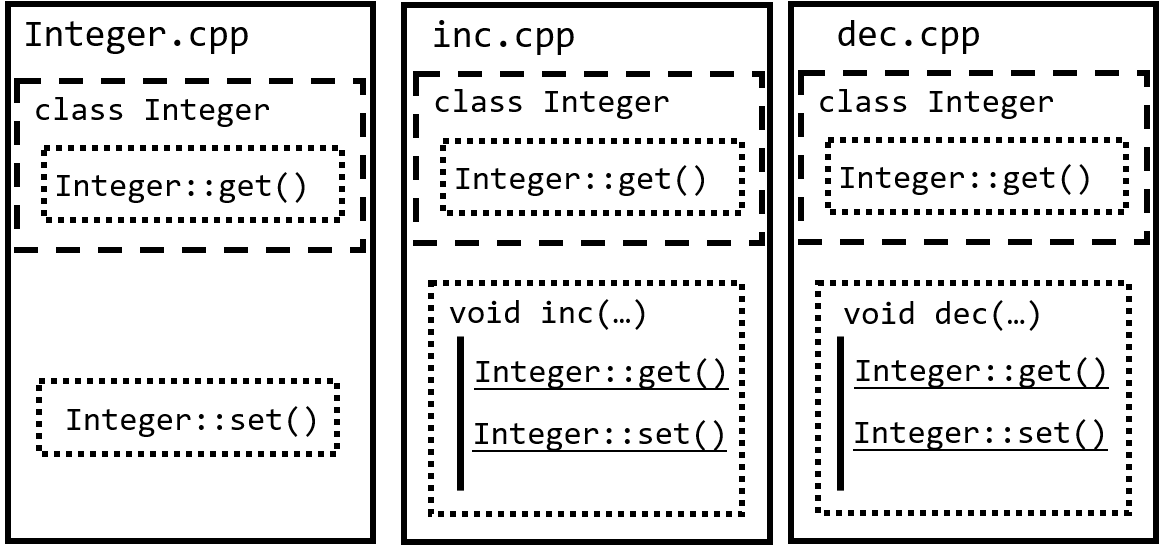
\includegraphics[scale=0.37]{fig/rc8link1}
\end{figure}

\end{frame}

\begin{frame}{On linking classes}
Pairs of the same color are linked together:
\begin{figure}
\centering
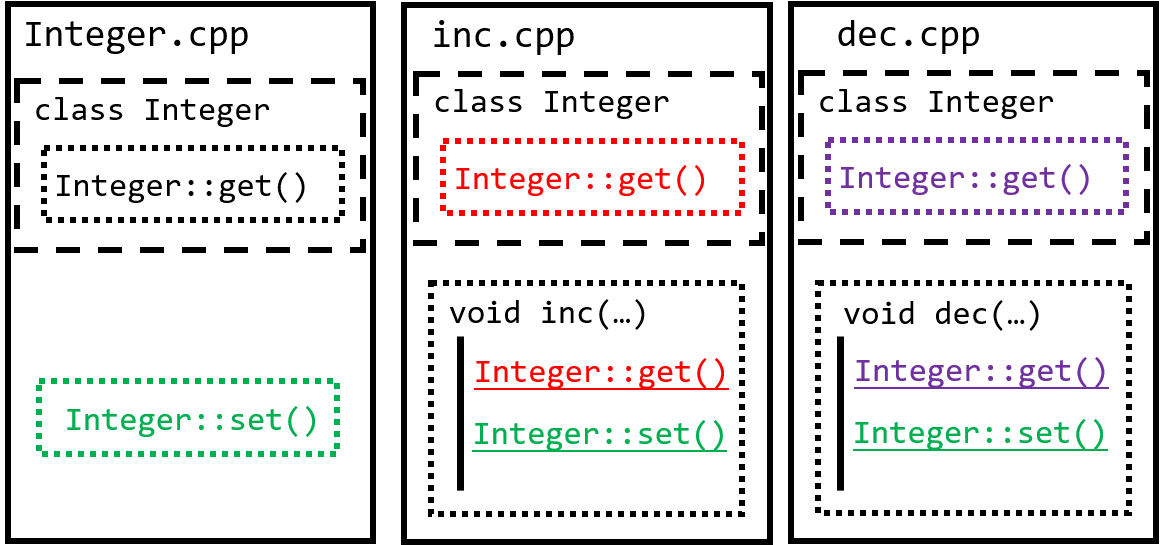
\includegraphics[scale=0.37]{fig/rc8link2}
\end{figure}
\end{frame}

\begin{frame}{On linking classes}
Thus the guideline is very simple:
\begin{itemize}
\item Methods defined inside the class decls are linked internally.
\item Methods defined in a separate \texttt{.cpp} source file are linked as if they are usual functions.
\end{itemize}
From a performance point of view, writing a definition of method inside the class declaration implies that the method is very simple. So instead of generating a function call whenever used the compiler will try to copy the code to each place it is used, avoiding the overhead of calling a function. This is called \textit{inlining}. 

\vspace{0.05in}
A remark we haven't made yet is \textit{abstraction always have an overhead}, a cost that we must endure to enable better flexibility. For classes, function calling mechanism is the overhead. Naturally people would want them both, i.e. ``zero cost abstraction". The way C++ achieves it is through allowing compiler to heavily optimize your code, and inlining methods is one major technique.
\end{frame}